\documentclass[11pt]{report}

\usepackage{epsf,amsmath,amsfonts}
\usepackage{graphicx}

\setlength{\textwidth}{6.5in}
\setlength{\oddsidemargin}{0in}
\setlength{\evensidemargin}{0in}
\setlength{\textheight}{8.5in}
\setlength{\topmargin}{0in}

\begin{document}

\title{
Requirements and Design\\
Tensor Operators}
\author{MPAS Development Team}

\maketitle
\tableofcontents

%-----------------------------------------------------------------------

\chapter{Summary}

The computation of the stress tensor and the divergence of the stress tensor are required for turbulence closures and the sea-ice momentum equation.  These operations on an unstructured grid are significantly more complicated than on a quadrilateral grid.  Here we provide algorithms to compute the strain rate tensor and the divergence of any symmetric rank-2 tensor . The stress tensor is related to the strain rate tensor through a constitutive relation that is not specified herein.  Analytic test cases are provided to validate the discrete.


%figure template
%\begin{figure}
%  \center{\includegraphics[width=14cm]{./Figure1.pdf}}
%  \caption{A graphical representation of the discrete boundary.}
%  \label{Figure1}
%\end{figure} 

%-----------------------------------------------------------------------

\chapter{Requirements}

\section{Requirement: Strain rate tensor}
Date last modified: 4/23/2013 \\
Contributors: Mark Petersen \\

 Given a discrete horizontal velocity field on the edges of an unstructured C-grid, compute the strain rate tensor 
\begin{equation}
\dot{\epsilon}_{ij} = \frac{1}{2}\left(\frac{\partial u_i}{\partial x_j} 
                                     + \frac{\partial u_j}{\partial x_i}\right).
\end{equation}


\section{Requirement: Divergence of a tensor}
Date last modified: 4/23/2013 \\
Contributors: Mark Petersen \\

Given a rank-2, symmetric tensor, $\sigma_{ij}$, at the edges of an unstructured C-grid, compute $\nabla\cdot\sigma$, the divergence of the tensor.  The output is a rank-1 tensor measured in $\mathbb{R}^3$.

\section{Requirement: Quantities must be available at all locations}
Date last modified: 4/23/2013 \\
Contributors: Mark Petersen \\

The strain rate tensor and tensor divergence must be available at cell centers, vertices, and edges.  One location may be the primary location, and others may be computed through interpolation.

\section{Requirement: Quantities must be available in $\mathbb{R}^3$ and $\mathbb{R}^2$ forms.}
Date last modified: 4/23/2013 \\
Contributors: Mark Petersen \\

The $\mathbb{R}^3$ form should be measured in Cartesian $(x,y,z)$ and lie in the tangent plane of an embedded surface (such as the surface of a sphere). In the $\mathbb{R}^2$ form, the local vertical direction is discarded and a new coordinate system spanning $\mathbb{R}^2$ is chosen.  The $\mathbb{R}^3$ form is preferred because typical global $\mathbb{R}^2$ coordinate systems, such as latitude-longitude coordinates, have pole problems.

\section{Requirement: Validation with analytic test functions}
Date last modified: 4/23/2013 \\
Contributors: Mark Petersen \\

Analytic test functions and solutions should provided in a testing subroutine for both Cartesian and spherical geometries.  These will be sufficiently general to fully exercise the numerical discretization.  This should include an arbitrary rotation with respect to the primary axes, and complex enough so that the divergence is not a constant.  For a fixed domain size, the root-mean-squared error should converge towards zero with a fixed order as grid-cell size decreases.  The required order of convergence is unknown.


%-----------------------------------------------------------------------

\chapter{Algorithmic Formulations}

\section{Design Solution: Strain rate tensor}
Date last modified: 4/23/2013 \\
Contributors: Mark Petersen \\

The strain rate tensor is an important operator for many applications.  In CICE, the stress tensor is computed from the strain rate tensor in each grid cell with a system of ODEs \cite[section 3.4]{CICE_manual_4.1}.  The computation of the stress tensor depends on the details of the model.  For example, they differ between viscous-plastic and elastic-viscous-plastic in CICE.  Computation of the strain rate tensor is a general operation, and can be placed in the operators subdirectory so it may be used by all MPAS cores.

The continuous strain rate tensor in Cartesian coordinates is
\begin{equation}
\dot{\epsilon}_{ij} = \frac{1}{2}\left(\frac{\partial u_i}{\partial x_j} 
                                     + \frac{\partial u_j}{\partial x_i}\right),
\end{equation}
where ${\bf u} = (u_1,u_2,u_3)$ is the velocity measured in Cartesian coordinates $(x_1,x_2,x_3)$.  In an arbitrary reference frame the strain rate tensor may be written using the Jacobian operator $J=\nabla {\bf u}$ as
\begin{equation}
{\bf\dot{\epsilon}} = \nabla_s {\bf u} \equiv \frac{1}{2}\left(J + J^T\right),
\end{equation}
where $\nabla_s$ denotes the symmetric gradient operator.  The weak form of the gradient, in continuous form, over a control surface $A$  is
\begin{equation}
\label{cont weak strain rate tensor}
\nabla {\bf u}
= \lim_{A\rightarrow(x,y)} \frac{1}{\tilde{A}} 
\int_{\partial A}
  {\bf n}\otimes{\bf u} \; dl
\end{equation}
\cite[equation 22]{Ringler06unpub} where $\tilde{A} = \int_A dA$ is the area, $dl$ is an increment along the boundary $\partial A$, and ${\bf n}$ is a unit vector normal to the boundary (Figure \ref{fig:2D domain}).  {\it Mark: I need to find a published reference for (\ref{cont weak strain rate tensor})}  The symbol $\otimes$ is the tensor product, which is the same as an outer product for two vectors.  In two-dimensional Cartesian space, ${\bf n}$ and ${\bf u}$ are both 2x1 vectors, and 
\begin{equation}
{\bf n}\otimes{\bf u} 
= \left( \begin{array}{c} n_1 \\ n_2 \end{array}   \right)
  \left( \begin{array}{cc} u_1 &  u_2 \end{array} \right)
= \left( \begin{array}{cc} n_1 u_1 & n_1 u_2 \\  n_2 u_1 & n_2 u_2 \end{array}   \right).
\end{equation}

\begin{figure}[htbp]
 \center
 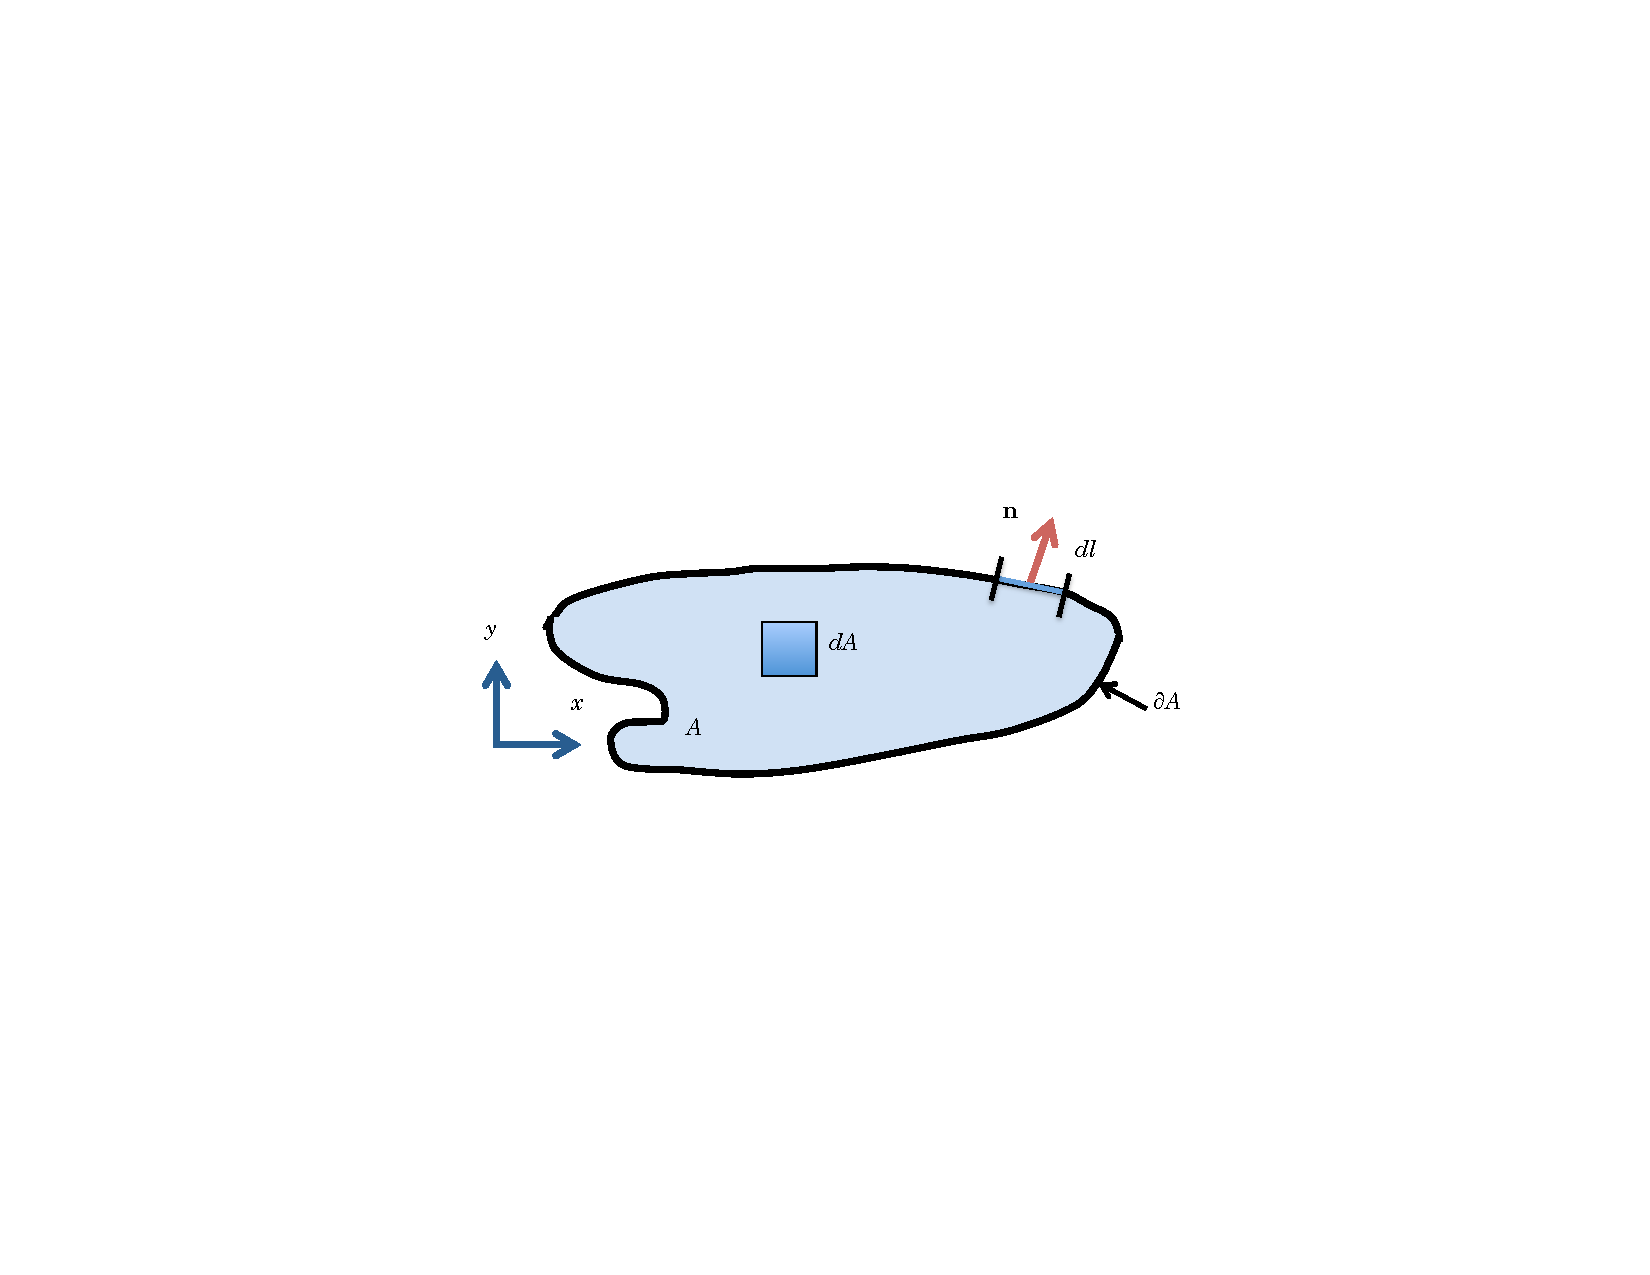
\includegraphics[trim=3.2in 3.2in 3.0in 3.5in, clip=true, scale=0.8]{f/A_surface.pdf}
 \caption{Two-dimensional surface $A$.}
 \label{fig:2D domain}
\end{figure}

The discrete form of (\ref{cont weak strain rate tensor}), where the control surface is a single cell, is
\begin{equation}
\label{cell strain rate tensor}
\left[\nabla {\bf u} \right]_i
= 
\frac{1}{A_i} 
\sum_{e\in EC(i)}{
  {\bf n}_e\otimes{\bf u}_e \; l_e },
\end{equation}
where $A_i$ is the area of cell $i$; $n_e$ is the unit vector normal to the edge $e$ measured in $\mathbb{R}^3$. Note that $n_e$ lies in the  tangent plane of the domain being used; $\bf{u_e}$ is the velocity vector at edge $e$ measured in $\mathbb{R}^3$; $l_e$ is the length of the edge, and $EC(i)$ is the set of edges surrounding cell $i$.  In the MPAS-Ocean code the velocity at an edge is written as 
\begin{eqnarray}
{\bf u}_e = u_e {\bf n}_e + v_e \tilde{\bf n}_e,
\end{eqnarray}
where $u_e$ is the \verb|normalVelocity| variable, $v_e$ is the \verb|tangentVelocity| variable.  Here $\tilde{\bf n}_e$ is the unit tangent vector on an edge,
\begin{eqnarray}
{\bf n}_e = \frac{{\bf x}_{i2}-{\bf x}_{i1}}{\left||{\bf x}_{i2}-{\bf x}_{i1}\right||}
  = \frac{1}{d_e} \sum_{i\in CE(e)}n_{e,i}{\bf x}_{i} 
\\
 \tilde{\bf n}_e = \frac{{\bf x}_{v2}-{\bf x}_{v1}}{\left||{\bf x}_{v2}-{\bf x}_{v1}\right||}
  = \frac{1}{l_e} \sum_{v\in VE(e)}n_{e,v}{\bf x}_{v},
\end{eqnarray}
where ${\bf x}$ provide locations of cell centers and vertices, $d_e$ is the distance between cell centers, and $n_{e,i}$ and $n_{e,v}$ provide an sign convention based on the ordering of cells and vertices on an edge.  Continuing from (\ref{cell strain rate tensor}), the velocity gradient is computed as
\begin{equation}
\label{cell strain rate tensor uv}
\left[\nabla {\bf u} \right]_i
= 
\frac{1}{A_i} 
\sum_{e\in EC(i)}{\left(
  u_e{\bf n}_e\otimes{\bf n}_e 
 +v_e{\bf n}_e\otimes\tilde{\bf n}_e 
\right)l_e },
\end{equation}
and the symmetric strain rate tensor as
\begin{equation}
\label{cell strain rate tensor sym}
\left[\dot\epsilon  \right]_i
= 
\left[\nabla_s {\bf u} \right]_i
= 
\left[\nabla {\bf u} \right]_i
+
\left[\nabla {\bf u} \right]^T_i.
\end{equation}

This algorithm computes a cell-centered strain rate measured in measured in $\mathbb{R}^3$ given a velocity field at edges.  This output may then be interpolated to edges or vertices, and rotated to a 2D symmetric tensor aligned with edges or an arbitrary reference frame.  Boundary conditions are simple; velocities at a land boundary are zero upon input.  If prognostic velocities are native to vertices or cell centers, as may be the case in MPAS-CICE, they must be interpolated to edges, and zeroed at land-boundary edges, before computing the strain rate.

\newpage
\section{Design Solution: Divergence of a tensor}
Date last modified: 4/23/2013 \\
Contributors: Mark Petersen \\

The weak form of the divergence of any symmetric tensor ${\mathbf F}$ is 
\begin{equation}
\label{cont div}
\nabla \cdot \mathbf{F} 
= 
\lim_{A\rightarrow(x,y)} \frac{1}{\tilde{A}} 
\int_{\partial A}
  {\bf n}\cdot{\mathbf F} \; dl
\end{equation}
in continuous form.  The divergence operator reduces the rank of $\mathbf{F}$ by 1.  In discrete form, the divergence of a rank-1 tensor (i.e. a vector) is
\begin{equation}
\label{discrete div}
[\nabla \cdot \mathbf{F}_:]_{i} = \frac{1} {A_i} \sum\limits_{e \in EC(i)} {n_{e,i} \, F_e \, l_e},
\end{equation}
where the operator computes a cell-centered divergence from a tensor field defined at edges. Here $F_e$ is the vector component normal to the edge, and $n_{e,i}$ indicates the sign of the vector at edge $e$ with respect to cell $i$.  The general discrete formulation of the divegence of a tensor is
\begin{equation}
\label{discrete div tensor}
[\nabla \cdot \mathbf{F}_:]_{i} = \frac{1} {A_i} \sum\limits_{e \in EC(i)} {\bf n}_e\cdot\mathbf{F}_e \; l_e.
\end{equation}

For the applications in this design document, tensor divergence reduces a rank-2 symmetric $\mathbb{R}^3$ tensor (written as a $3\times 3$ matrix) to a rank-1 $\mathbb{R}^3$ tensor (i.e. a vector in $\mathbb{R}^3$).  Common examples of rank-2 symmetric $\mathbb{R}^3$ tensors in fluid mechanics are the strain rate tensor and the stress tensor.  The discrete divergence begins with edge quantities and produces a cell-centered quantity.  Additional subroutines will interpolate the vector to edges or vertices, and rotate the vector into any 2D reference frame needed.  For example, the component of the stress tensor normal to an edge is simply
\begin{equation}
{\bf n}_e\cdot[\nabla \cdot \sigma]_{e}.
\end{equation}

Boundary conditions for $\sigma$ at land edges are not necessarily zero, as there can be shear stress at the wall.  If the stress tensor is native to vertices, interpolation to edge values may be done by simple averaging.  If the stress tensor is native to cell centers, the stress tensor at the land cell is zero, so a simple average to the edge will be half the value of the ocean cell.

%-----------------------------------------------------------------------

\chapter{Design and Implementation}

\section{Implementation: Workflow for MPAS-O turbulence closure}
Date last modified: 4/23/2013 \\
Contributors: Mark Petersen \\

An example of a workflow for an MPAS-Ocean turbulence closure using the strain rate and stress tensor is as follows.  The turbulence closure routine may be executed on cell centers, vertices, or edges.  A graphical version is shown in figure \ref{fig:mpaso_tensor_workflow}
\\
\begin{tabular}{ |l| l| l| }
\hline
  {\bf subroutine} &  {\bf input} &  {\bf output} \\
\hline
\verb|mpas_tangential_velocity|  & $u_e$ \verb|normalVelocity| & $v_e$ \verb|tangentVelocity|  \\
\verb|mpas_strain_rate_R3Cell|   & $u_e$ \verb|normalVelocity| & $\left[\dot\epsilon  \right]_i$ \verb|strainRateR3Cell|\\
&  $v_e$ \verb|tangentVelocity| &\\
interpolate to edge or vertex and 2D if desired &  $\left[\dot\epsilon  \right]_i$ &  $\left[\dot\epsilon  \right]_e$ or $\left[\dot\epsilon  \right]_v$\\
turbulence closure: compute stress tensor &  $\left[\dot\epsilon  \right]_:$ &  $\left[\sigma  \right]_:$\\
interpolate to edge, if needed   & $\left[\sigma  \right]_:$&  $\left[\sigma  \right]_e$\\
\verb|mpas_divergence_of_tensor_R3Cell|   &  $\left[\sigma  \right]_e$ \verb|strainRateR3Edge|& $[\nabla \cdot \sigma]_{i}$ \verb|divTensorR3Cell|\\
\verb|mpas_vector_R3Cell_to_2DEdge|  &  $[\nabla \cdot \sigma]_{i}$ \verb|divTensorR3Cell| & ${\bf n}_e\cdot[\nabla \cdot \sigma]_{e}$, ${\bf \tilde n}_e\cdot[\nabla \cdot \sigma]_{e}$ \\
add $[\nabla \cdot \sigma]$ terms to momentum equation & & \\
\hline
\end{tabular}

\begin{figure}[htbp]
 \center
 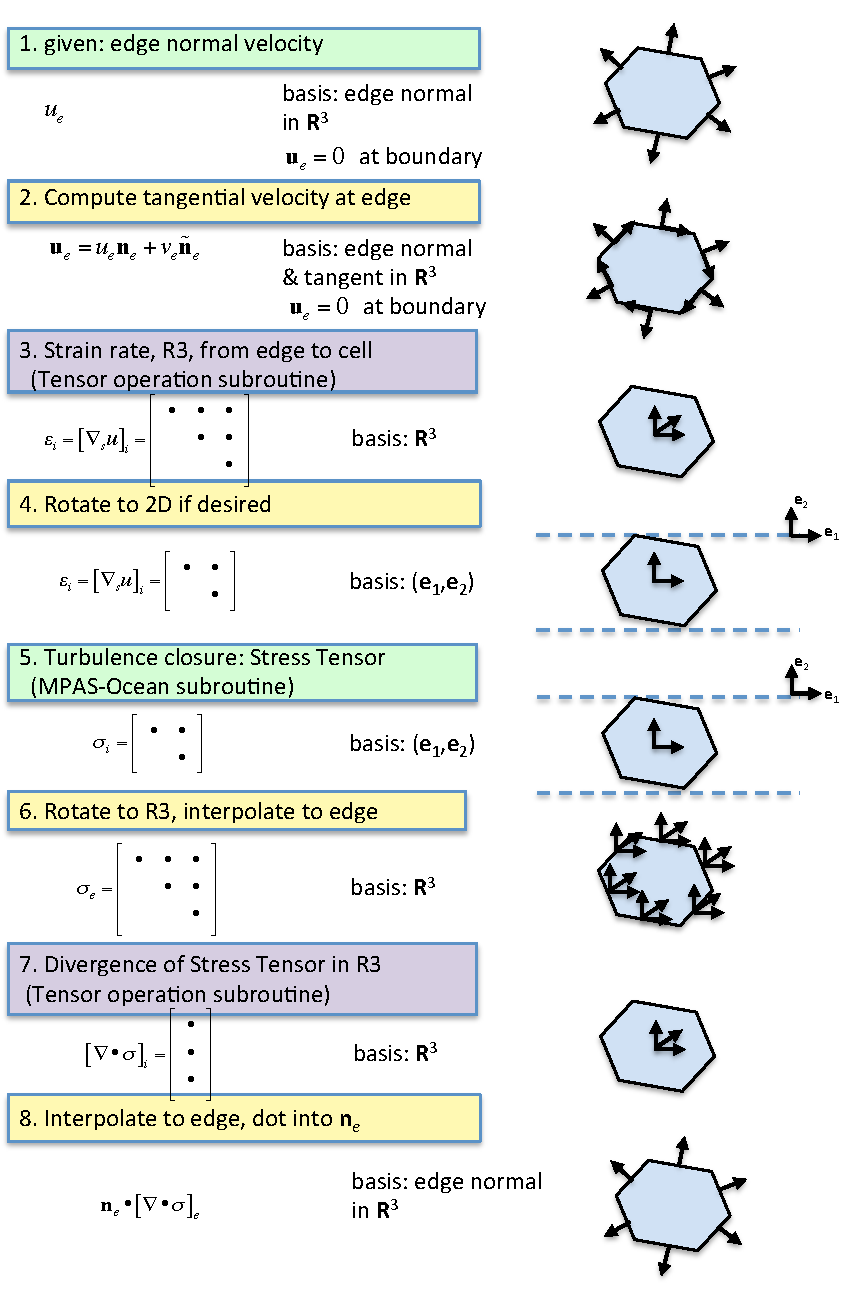
\includegraphics[scale=0.9]{f/mpaso_tensor_workflow.pdf}
 \caption{MPAS-Ocean workflow}
 \label{fig:mpaso_tensor_workflow}
\end{figure}


\newpage

\section{Implementation: Workflow for MPAS-CICE}
Date last modified: 4/23/2013 \\
Contributors: Mark Petersen \\

The formulation for strain rate and tensor divergence provided in this library always computes from edges to cell centers.  However, MPAS-CICE developers are free to solve the stress tensor and momentum equations at the location of their choice, and in the local coordinate system of their choice, by using the provided interpolation and rotation subroutines. For example, the following is a workflow for solving the momentum equation at vertices in a local 2D latitude-longitude coordinate system.  This is the same as the current CICE code when on quadrilateral cells.  In addition, the constitutive relation between strain rate and stress is solved in the 2D form, as in CICE.  An example of the MPAS-CICE workflow for three-dimensional tensor operations is as follows, and is shown graphically in figure \ref{fig:mpasCICE_tensor_workflow1}.  Alternately, all tensor operations could be conducted in 2D, as shown in figure \ref{fig:mpasCICE_tensor_workflow2}.\\
\begin{tabular}{ |l| l| l| }
\hline
  {\bf subroutine} &  {\bf input} &  {\bf output} \\
\hline
{\bf solve momentum equation} at vertices &$[\nabla \cdot \sigma]_v$ (2D) & $u_v$, $v_v$\\
interpolate to edge, expand to R3 & $u_v$, $v_v$ & ${\bf u}_e$ \\
\verb|mpas_strain_rate_R3Cell|   & ${\bf u}_e$ & $\left[\dot\epsilon  \right]_i$ \\
rotate to 2D &  $\left[\dot\epsilon  \right]_i$ (R3) &  $\left[\dot\epsilon  \right]_i$ (2D)\\
{\bf compute stress tensor in 2D} &  $\left[\dot\epsilon  \right]_i$ (2D) &  $\left[\sigma  \right]_i$ (2D)\\
rotate to R3, interpolate to edge  & $\left[\sigma  \right]_i$ (2D) &  $\left[\sigma  \right]_e$ (R3) \\
\verb|mpas_divergence_of_tensor_R3Vertex|   &  $\left[\sigma  \right]_e$ \verb|strainRateR3Edge|& $[\nabla \cdot \sigma]_v$ \verb|divTensorR3Vertex|\\
rotate to 2D for momentum forcing &  $[\nabla \cdot \sigma]_v$ (R3) & $[\nabla \cdot \sigma]_v$ (2D) \\
\hline
\end{tabular}
\vspace{8pt}

The MPAS-CICE routines required for this workflow are to solve the momentum equation and compute the stress tensor.  These operations are both point-wise (i.e., they do not involve neighbors given these inputs), and so the subroutines could in general solve these on cells centers, vertices, or edges.  

If the momentum equation is solved on edges or vertices, boundary conditions for velocity is simply zero on land boundaries.  If the momentum equation is solved at cell centers, the velocity interpolated to the edge could be set to zero before the advection and strain rate are computed.  For the strain rate and stress tensor, use a land-cell value of zero when averaging from cell centers to edges, and use a straight average from vertices to edges.

\begin{figure}[htbp]
 \center
 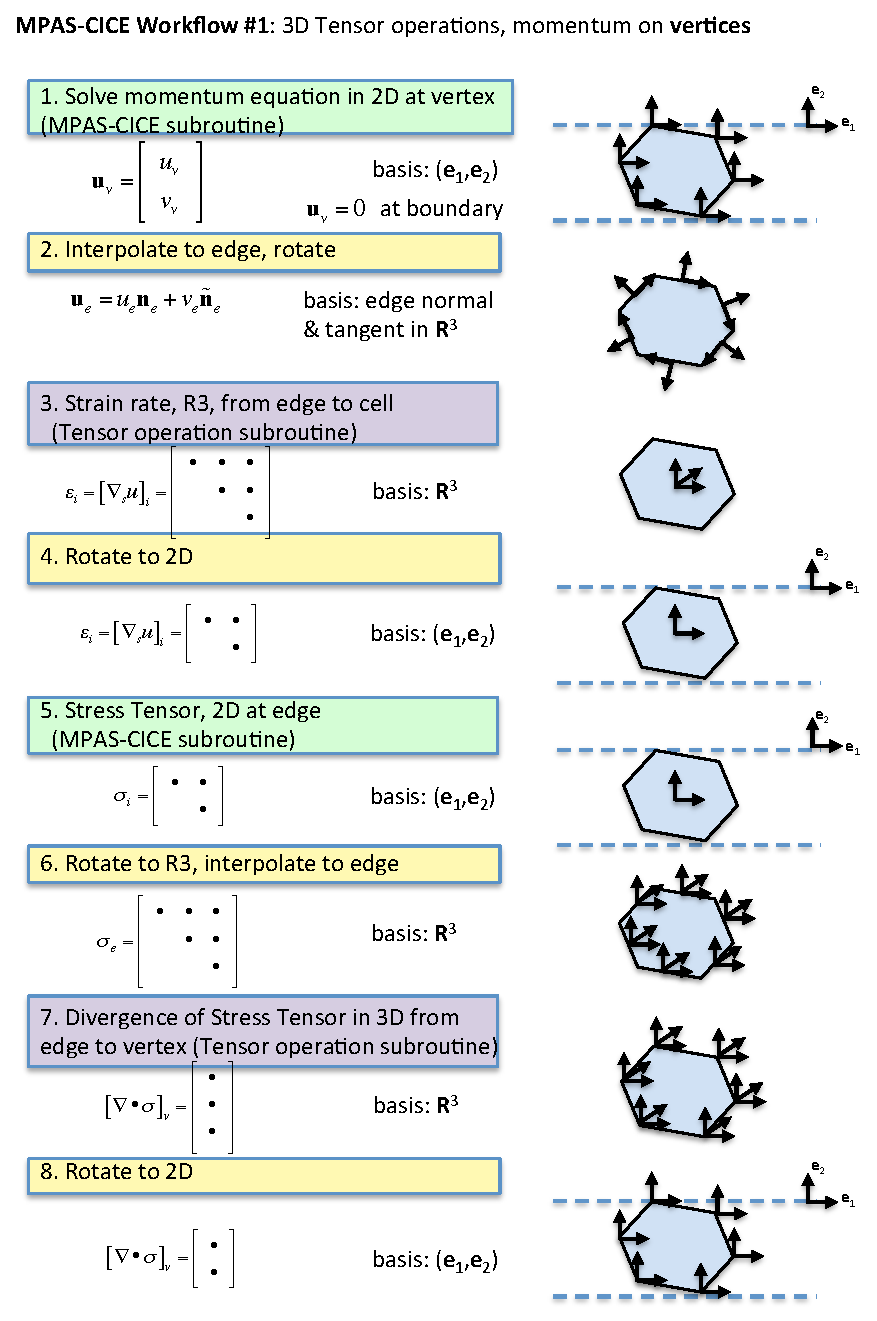
\includegraphics[scale=0.9]{f/mpasCICE_tensor_workflow1.pdf}
 \caption{MPAS-CICE workflow, tensor operations in R3}
 \label{fig:mpasCICE_tensor_workflow1}
\end{figure}


\begin{figure}[htbp]
 \center
 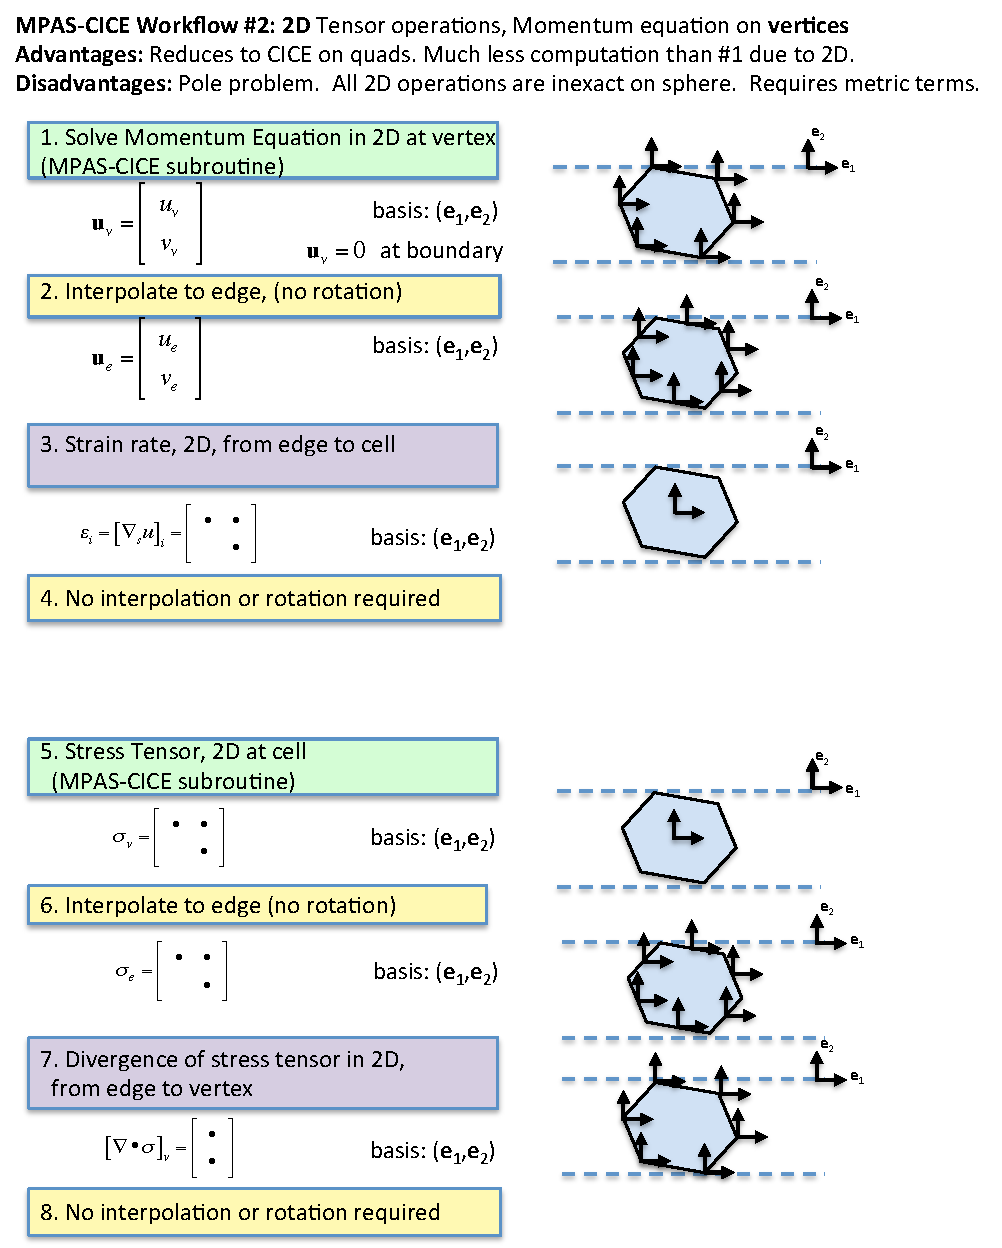
\includegraphics[scale=0.9]{f/mpasCICE_tensor_workflow2.pdf}
 \caption{MPAS-CICE workflow, tensor operations in 2D}
 \label{fig:mpasCICE_tensor_workflow2}
\end{figure}


%-----------------------------------------------------------------------

\chapter{Testing and Validation}

\section{Testing functions for strain rate and its divergence on a plane}
Date last modified: 4/23/2013 \\
Contributors: Mark Petersen \\

The following analytic test cases may be used to test the tensor operators on any two-dimension Cartesian domain, including quads, hexes, and variable resolution meshs.  There are presently no test cases for a sphere.  All cases are implemented in the subroutine \verb|mpas_test_tensor|.  It is clear that some later test cases are a superset of earlier ones.  For example, the linear case is the power function with $n=1$.  But the earlier simple cases are instructional and useful for debugging, and so are included here and in the code.

The constant coefficients $c_n$ and $c_s$ are for the normal and shear components of the strain, respectively.  When velocities are aligned with an axis, like in cases \ref{linear_x}, \ref{linear_y}, \ref{power_x}, and \ref{power_y}, the normal strain appears on the diagonals of the strain rate tensor, and the shear appears on the off-diagonals.  However, for arbitrary rotations, both components appear in all the elements of the strain rate tensor.

\subsection{Linear in x\label{linear_x}}
\begin{eqnarray}
{\bf u}(x,y) &=& \left( \begin{array}{c} c_n \\ c_s \end{array}   \right)x \\
\nabla{\bf u}^* &=& \left( \begin{array}{c} \partial_x \\ \partial_y \end{array}   \right) \left( \begin{array}{cc} c_nx & c_sx \end{array}   \right)
 =  \left( \begin{array}{cc} c_n & c_s \\ 0 & 0 \end{array}   \right) \\
\nabla_s{\bf u}^* &=&  \left( \begin{array}{cc} c_n & \frac{1}{2}c_s \\ \frac{1}{2}c_s & 0 \end{array}   \right) \\
\nabla\cdot\left(\nabla_s{\bf u}\right) &=&  \left( \begin{array}{cc} 0 & 0 \end{array}   \right)
\end{eqnarray}

\subsection{Linear in y\label{linear_y}}
\begin{eqnarray}
{\bf u}(x,y) &=& \left( \begin{array}{c} -c_s \\ c_n \end{array}   \right)y \\
\nabla{\bf u}^* &=& \left( \begin{array}{c} \partial_x \\ \partial_y \end{array}   \right) \left( \begin{array}{cc} -c_sy & c_ny \end{array}   \right)
 =  \left( \begin{array}{cc}  0 & 0 \\ -c_s & c_n  \end{array}   \right) \\
\nabla_s{\bf u}^* &=&  \left( \begin{array}{cc} 0 & -\frac{1}{2}c_s \\ -\frac{1}{2}c_s & c_n \end{array}   \right) \\
\nabla\cdot\left(\nabla_s{\bf u}\right) &=&  \left( \begin{array}{cc} 0 & 0 \end{array}   \right)
\end{eqnarray}

\subsection{Linear, rotated about an arbitrary angle $\theta_r$\label{linear_rotation}}
\begin{eqnarray}
{\bf u}(r,\theta;\theta_r) &=& r\cos{(\theta-\theta_r)} R_{\theta_r} \left( \begin{array}{c} c_n \\ c_s \end{array}   \right) = f{\bf g}
\end{eqnarray}
where 
\begin{eqnarray}
\label{def f}
f(r,\theta;\theta_r)&\equiv& r\cos{(\theta-\theta_r)},\\
\label{def g}
{\bf g}(\theta_r) &\equiv& R_{\theta_r} \left( \begin{array}{c} c_n \\ c_s \end{array}   \right) \\
&=& \left(\begin{array}{cc} \cos{\theta_r}& -\sin{\theta_r} \\
                          \sin{\theta_r}&  \cos{\theta_r}   \end{array}\right)
 \left( \begin{array}{c} c_n \\ c_s \end{array}   \right)\\
&=& \left(\begin{array}{c} c_n\cos{\theta_r} -c_s\sin{\theta_r} \\
                          c_n\sin{\theta_r} +  c_s \cos{\theta_r}   \end{array}\right)
\end{eqnarray}
Note that when $\theta_r=0$ this simplifies to case \ref{linear_x} and when $\theta_r=\pi/2$ this simplifies to case \ref{linear_y}.  Recall the trig identity
\begin{equation}
\cos{(a-b)} = \cos{a}\cos{b} + \sin{a}\sin{b}
\end{equation}
so that 
\begin{eqnarray}
f&\equiv& r\cos{(\theta-\theta_r)}\\
 &=& r\cos{\theta}\cos{\theta_r} + r\sin{\theta}\sin{\theta_r}\\
 &=& x\cos{\theta_r} + y\sin{\theta_r}.
\end{eqnarray}
Finally, the operators of interest for this test case are
\begin{eqnarray}
\nabla{\bf u}^* &=& \left( \nabla f \right) {\bf g}^* 
 = \left( \begin{array}{c} \cos{\theta_r} \\ \sin{\theta_r} \end{array}    \right)  
\left(\begin{array}{cc} g_1 & g_2  \end{array} \right)
= \left(\begin{array}{cc} g_1\cos{\theta_r} & g_2\cos{\theta_r} \\ g_1\sin{\theta_r} & g_2\sin{\theta_r}  \end{array} \right)\\
\nabla_s{\bf u}^* &=& \left(\begin{array}{cc} g_1\cos{\theta_r} & \frac{1}{2}\left( g_1\sin{\theta_r} + g_2\cos{\theta_r} \right)\\
                      (sym) & g_2\sin{\theta_r}  \end{array} \right)\\
\nabla\cdot\left(\nabla_s{\bf u}\right) &=&  \left( \begin{array}{cc} 0 & 0 \end{array}   \right).
\end{eqnarray}

\subsection{Power Function in x\label{power_x}}
\begin{eqnarray}
{\bf u}(x,y) &=& \left( \begin{array}{c} c_n \\ c_s \end{array}   \right)x^{n} \\
\nabla{\bf u}^* &=& \left( \begin{array}{c} \partial_x \\ \partial_y \end{array}   \right) \left( \begin{array}{cc} c_nx^{n} & c_sx^{n} \end{array}   \right)
 =  \left( \begin{array}{cc} c_n & c_s \\ 0 & 0 \end{array}   \right) nx^{n-1}\\
\nabla_s{\bf u}^* &=&  \left( \begin{array}{cc} c_n & \frac{1}{2}c_s \\ \frac{1}{2}c_s & 0 \end{array}   \right) nx^{n-1}\\
\nabla\cdot\left(\nabla_s{\bf u}\right) &=&  \left( \begin{array}{cc} \partial_x & \partial_y \end{array}   \right)
\left( \begin{array}{cc} c_n & \frac{1}{2}c_s \\ \frac{1}{2}c_s & 0 \end{array}   \right) nx^{n-1}
 = \left( \begin{array}{cc} c_n & \frac{1}{2}c_s \end{array}   \right) n(n-1)x^{n-2}
\end{eqnarray}

\subsection{Power Function in y\label{power_y}}
\begin{eqnarray}
{\bf u}(x,y) &=& \left( \begin{array}{c} -c_s \\ c_n \end{array}   \right)y^{n} \\
\nabla{\bf u}^* &=& \left( \begin{array}{c} \partial_x \\ \partial_y \end{array}   \right) \left( \begin{array}{cc} -c_sy & c_ny \end{array}   \right)
 =  \left( \begin{array}{cc}  0 & 0 \\ -c_s & c_n  \end{array}   \right) ny^{n-1}\\
\nabla_s{\bf u}^* &=&  \left( \begin{array}{cc} 0 & -\frac{1}{2}c_s \\ -\frac{1}{2}c_s & c_n \end{array}   \right) ny^{n-1}\\
\nabla\cdot\left(\nabla_s{\bf u}\right) &=&  \left( \begin{array}{cc} \partial_x & \partial_y \end{array}   \right) 
\left( \begin{array}{cc} 0 & -\frac{1}{2}c_s \\ -\frac{1}{2}c_s & c_n \end{array}   \right) ny^{n-1}
= \left( \begin{array}{cc} -\frac{1}{2}c_s & c_n \end{array}   \right) n(n-1)y^{n-2}
\end{eqnarray}

\subsection{Power Function, rotated about an arbitrary angle $\theta_r$\label{power_rotation}}
Using the definitions of f and g in (\ref{def f}-\ref{def g}),
\begin{eqnarray}
{\bf u}(r,\theta;\theta_r) &=& f^n{\bf g}\\
\nabla{\bf u}^* &=& \left( \nabla f^n \right) {\bf g}^* 
=  n f^{n-1} \nabla f {\bf g}^* 
 = n f^{n-1} \left( \begin{array}{c} \cos{\theta_r} \\ \sin{\theta_r} \end{array}    \right)  {\bf g}^* \\
\nabla_s{\bf u}^* &=&  n f^{n-1}
        \left(\begin{array}{cc} g_1\cos{\theta_r} & \frac{1}{2}\left( g_1\sin{\theta_r} + g_2\cos{\theta_r} \right)\\
                        (sym) & g_2\sin{\theta_r}  \end{array} \right)\\
\nabla\cdot\left(\nabla_s{\bf u}\right) &=&  \left( \begin{array}{cc} \partial_x & \partial_y \end{array}   \right)
n f^{n-1} \left(\begin{array}{cc} g_1\cos{\theta_r} & \frac{1}{2}\left( g_1\sin{\theta_r} + g_2\cos{\theta_r} \right)\\
                        (sym) & g_2\sin{\theta_r}  \end{array} \right)\\
 &=& n(n-1) f^{n-2} \left( \begin{array}{c} \cos{\theta_r} \\ \sin{\theta_r} \end{array}    \right)^*  
\left(\begin{array}{cc} g_1\cos{\theta_r} & \frac{1}{2}\left( g_1\sin{\theta_r} + g_2\cos{\theta_r} \right)\\
                        (sym) & g_2\sin{\theta_r}  \end{array} \right)\\
 &=& n(n-1) f^{n-2} \left(\begin{array}{c} 
   g_1\left(\cos^2{\theta_r} + \frac{1}{2}\sin^2{\theta_r}\right) + g_2\frac{1}{2}\cos{\theta_r}\sin{\theta_r} \\
   g_2\left(\sin^2{\theta_r} + \frac{1}{2}\cos^2{\theta_r}\right) + g_1\frac{1}{2}\cos{\theta_r}\sin{\theta_r} \\
\end{array} \right)^*
\end{eqnarray}

\subsection{Sine function, rotated about an arbitrary angle $\theta_r$\label{sine_rotation}}
Using the definitions of f and g in (\ref{def f}-\ref{def g}),
\begin{eqnarray}
{\bf u}(r,\theta;\theta_r) &=& \sin{\left(\frac{2\pi}{L}r\cos{(\theta-\theta_r)}\right)}
   R_{\theta_r} \left( \begin{array}{c} c_n \\ c_s \end{array}   \right) \\
&=& \sin{\left(\frac{2\pi}{L}f\right)}{\bf g} \\
\nabla{\bf u}^* &=& \frac{2\pi}{L}\cos{\left(\frac{2\pi}{L}f\right)}\left( \nabla f \right) {\bf g}^* \\
 &=& \frac{2\pi}{L}\cos{\left(\frac{2\pi}{L}f\right)}
\left( \begin{array}{c} \cos{\theta_r} \\ \sin{\theta_r} \end{array}    \right)  
\left(\begin{array}{cc} g_1 & g_2  \end{array} \right) \\
&=& \frac{2\pi}{L}\cos{\left(\frac{2\pi}{L}f\right)}
\left(\begin{array}{cc} g_1\cos{\theta_r} & g_2\cos{\theta_r} \\ g_1\sin{\theta_r} & g_2\sin{\theta_r}  \end{array} \right)\\
\nabla_s{\bf u}^* &=& \frac{2\pi}{L}\cos{\left(\frac{2\pi}{L}f\right)}
\left(\begin{array}{cc} g_1\cos{\theta_r} & \frac{1}{2}\left( g_1\sin{\theta_r} + g_2\cos{\theta_r} \right)\\
                      (sym) & g_2\sin{\theta_r}  \end{array} \right)\\
\nabla\cdot\left(\nabla_s{\bf u}\right) &=&  \left( \begin{array}{cc} \partial_x & \partial_y \end{array}   \right)
\frac{2\pi}{L}\cos{\left(\frac{2\pi}{L}f\right)}
\left(\begin{array}{cc} g_1\cos{\theta_r} & \frac{1}{2}\left( g_1\sin{\theta_r} + g_2\cos{\theta_r} \right)\\
                      (sym) & g_2\sin{\theta_r}  \end{array} \right)\\
&=& -\left(\frac{2\pi}{L}\right)^2
\sin{\left(\frac{2\pi}{L}f\right)}\left( \nabla f \right)^* 
\left(\begin{array}{cc} g_1\cos{\theta_r} & \frac{1}{2}\left( g_1\sin{\theta_r} + g_2\cos{\theta_r} \right)\\
                      (sym) & g_2\sin{\theta_r}  \end{array} \right)\\
&=& -\left(\frac{2\pi}{L}\right)^2
\sin{\left(\frac{2\pi}{L}f\right)}
\left( \begin{array}{c} \cos{\theta_r} \\ \sin{\theta_r} \end{array}    \right)  ^* 
\left(\begin{array}{cc} g_1\cos{\theta_r} & \frac{1}{2}\left( g_1\sin{\theta_r} + g_2\cos{\theta_r} \right)\\
                      (sym) & g_2\sin{\theta_r}  \end{array} \right)\\
&=& -\left(\frac{2\pi}{L}\right)^2
\sin{\left(\frac{2\pi}{L}f\right)}
\left(\begin{array}{c} g_1\cos^2{\theta_r} + \frac{1}{2}\left( g_1\sin^2{\theta_r} + g_2\cos{\theta_r}\sin{\theta_r} \right)\\
                       g_2\sin^2{\theta_r} + \frac{1}{2}\left( g_2\cos^2{\theta_r} + g_1\cos{\theta_r}\sin{\theta_r} \right) 
 \end{array} \right)^* 
\end{eqnarray}

\section{Testing functions for strain rate and its divergence on a sphere}
Date last modified: 4/23/2013 \\
Contributors: Mark Petersen \\

{\it Mark:} I have these written by hand, need to add in latex.

\bibliographystyle{alpha}
\bibliography{tensor_operations}



%-----------------------------------------------------------------------
\end{document}
